\documentclass{standalone}
\usepackage{tikz}
\usepackage{tkz-euclide}
\usepackage{ctex}
\pagestyle{empty}
\setCJKmainfont{Noto Serif CJK SC}
\usepackage{siunitx,chemmacros,chemfig}
\setchemfig{bond offset = 0pt}
\chemsetup[orbital]{
  overlay,
  opacity=0.5,
  sp/scale=2.0,
  s/color=blue!50,
  s/scale=2.5
}
\begin{document}
\small
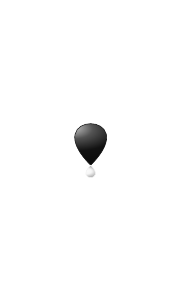
\begin{tikzpicture}
  \useasboundingbox(-0.8,-1.5)rectangle(0.8,1.5);
  % \draw[very thin](0,0)--(0,1.5)(0,0)--(-19.5:1.5);
\node {\chemfig{
  {\orbital{sp}}%{\orbital[angle=-19.5]{sp}}{\orbital[angle=210]{sp}}{\orbital[angle=240]{sp}}
}};
% \draw[very thin](0,0.5)arc(90:-19.5:0.5)node[midway,above right]{\ang{109;28;}};
\end{tikzpicture}
\end{document}